% Template created by Karol Kozioł (www.karol-koziol.net) for ShareLaTeX

\documentclass[letterpaper,9pt,fleqn]{extarticle}
\usepackage[utf8]{inputenc}
\usepackage[T1]{fontenc}

\usepackage[]{graphicx}
\usepackage{caption}
\usepackage{subcaption}

\usepackage{xcolor}
\usepackage{tikz}
%\usepackage{pgfplots}
%\pgfplotsset{width=5cm,compat=1.9}
\usepackage{hyperref}
\usetikzlibrary{shapes.geometric}
\usetikzlibrary{calc}
\usepackage{array}   % for \newcolumntype macro
\usepackage{fourier}
\usepackage{graphicx,nicefrac}
\usepackage{isomath,upgreek,comment}
\usepackage{pdfpages}
\usepackage{tkz-euclide}
%\usetkzobj{all}

\usepackage[activate={true,nocompatibility},final,tracking=true,kerning=true,factor=1100,stretch=10,shrink=10]{microtype}
\usepackage[american]{babel}

\usepackage{amstext} % for \text macro
\usepackage{array}   % for \newcolumntype macro
\newcolumntype{L}{>{$}l<{$}} % math-mode version of "l" column type

\newcommand{\dom}{\mathrm{dom}} 
\newcommand{\range}{\mathrm{range}} 
\newcommand{\zero}{\mathrm{zero}} 
\newcommand{\reals}{\mathbf{R}} 
\newcommand{\integers}{\mathbf{Z}} 
\newcommand{\ssep}{\mid}
\newcommand{\arcsec}{\mathrm{arcsec}}
\newcommand{\arccsc}{\mathrm{arccsc}}
\newcommand{\arccot}{\mathrm{arccot}}

\usepackage{amsmath,amssymb,textcomp}
\everymath{\displaystyle}

%\usepackage{times}
%\renewcommand\familydefault{\sfdefault}
%\usepackage{tgheros}
%\usepackage[defaultmono,scale=0.85]{droidmono}
%\usepackage{fourier}
\usepackage{multicol}
\setlength{\columnseprule}{0pt}
\setlength{\columnsep}{20.0pt}


\usepackage{geometry}
\geometry{letterpaper,left=5mm,right=5mm,top=5mm,bottom=5mm}

\linespread{1.3}


% custom title
\makeatletter
\renewcommand*{\maketitle}{%
\noindent
\begin{minipage}{0.4\textwidth}

\begin{tikzpicture}
\node[rectangle,rounded corners=6pt,inner sep=10pt,fill=blue!50!black,text width= 0.95\textwidth] {\color{white}\Huge \@title};
\end{tikzpicture}
\end{minipage}
\hfill
\begin{minipage}{0.55\textwidth}

\begin{tikzpicture}
\node[rectangle,rounded corners=3pt,inner sep=10pt,draw=blue!50!black,text width= 0.95\textwidth] {\LARGE \@author};
\end{tikzpicture}
\end{minipage}
\bigskip\bigskip
}%
\makeatother

% custom section
\usepackage[explicit]{titlesec}
\newcommand*\sectionlabel{}
\titleformat{\section}
  {\gdef\sectionlabel{}
   \normalfont\sffamily\Large\bfseries\scshape}
  {\gdef\sectionlabel{\thesection\ }}{0pt}
  {
\noindent
\begin{tikzpicture}
\node[rectangle,rounded corners=3pt,inner sep=4pt,fill=blue!50!black,text width= 0.95\columnwidth] {\color{white}\sectionlabel#1};
\end{tikzpicture}
  }
\titlespacing*{\section}{0pt}{15pt}{10pt}


% custom footer
\usepackage{fancyhdr}
\makeatletter
%\pagestyle{fancy}
\fancyhead{}
%\fancyfoot[C]{\footnotesize \textcopyright\ \@date\ \ \@author}
\renewcommand{\headrulewidth}{0pt}
\renewcommand{\footrulewidth}{0pt}
\makeatother

\newcommand{\term}{ Fall }

\newcommand{\myclass}{ MATH 103}
\title{\myclass, \term \the\year}
\author{Barton Willis, PhD, Professor of Mathematics}




\begin{document}

%\maketitle

\begin{multicols*}{3}



\section*{Greek Characters}
\vspace{-0.35in}



\begin{tabular}{|L | L| L|} \hline
\mbox{Name} & \mbox{Symbol} & \mbox{Typical use(s)} \\ \hline
\mathrm{alpha} & \alpha  & \mbox{angle, constant} \\
\mathrm{beta} & \beta  & \mbox{angle, constant}  \\ 
\mathrm{gamma} & \gamma & \mbox{angle, constant} \\
%\mathrm{delta} & \delta  & \mbox{ limit definition}\\
\mathrm{epsilon} & \epsilon  \mbox{ or } \varepsilon & \mbox{angle, constant} \\
\mathrm{theta}  & \theta  \mbox{ or } \vartheta & \mbox{angle, constant}\\ 
%\mathrm{lambda} & \lambda & \mbox{Lagrange multiplier} \\
\mathrm{pi} & \pi \mbox{ or } \uppi & \mbox{circular constant} \\
\mathrm{phi} & \phi \mbox{ or } \varphi  & \mbox{angle, constant} \\

\hline
\end{tabular}

\vspace{-0.1in}

\section*{Named Sets}

\vspace{-0.35in}
\begin{tabular}{|L | L |} \hline 
\mathrm{empty\,\, set} & \varnothing \\ 
 \mathrm{real\,\, numbers} & \mathbf{R} \\
  \mathrm{ordered \, \, pairs \,\,  of \,\, reals}  & \mathbf{R}^2 \\
  %\mathrm{ordered \, \, triples }  & \mathbf{R}^3 \\
  \mathrm{integers } & \mathbf{Z} \\
  \mathrm{positive \,\,  integers } & \mathbf{Z}_{>0} \\ 
  \mathrm{positive \,\, real \,\,  numbers} & \mathbf{R}_{>0} \\ 
  \hline
  \end{tabular}

\section*{Set Symbols}
\vspace{-0.35in}
%The \emph{union} is the members that belong to both sets; the \emph{intersection} are the members that belong to both sets.

\begin{tabular}{|L | L|} \hline
\mbox{Meaning}  & \mbox{Symbol} \\ \hline
\mathrm{is \,\, a \,\, member} & \in \\
\mathrm{subset}       & \subset \\
\mathrm{intersection} & \cap \\
\mathrm{union} & \cup  \\ 
\mathrm{set \,\,  minus}  & \setminus \\ \hline
\end{tabular}

%\vspace{0.1in}

%\noindent For sets \(A\) and \(B\), the statement \(A \subset B\) is true
%when every member of \(A\) is a member of \(B\).
\section*{Intervals}
\vspace{-0.35in}
\begin{minipage}[c]{0.333\textwidth}
For numbers \(a\) and \(b\), we define the intervals:
\begin{align*}
 (a,b) &= \left\{x \in \reals \ssep a < x < b \right\}  \\
  [a,b) &= \{x  \in \reals  \ssep a \leq  x < b \} \\
   (a,b] &= \{x  \in \reals \ssep a <  x \leq  b \} \\
    [a,b]  &= \{x  \in \reals \ssep a \leq  x \leq  b \} \\
    (-\infty, a) &= \{x \mid x < a \} \\
    (-\infty, a] &= \{x \mid x \leq  a \} \\
  (a, \infty)  &= \{x \mid a < x  \} \\
   [a, \infty)  &= \{x \mid a \leq  x  \} \\
\end{align*}  
\end{minipage}
\vspace{-0.35in}

\section*{Logic Symbols}
\vspace{-0.35in}
%In mathematical logic, \(\ma{True or  True} \) is true.
\begin{tabular}{|L | L|} \hline 
\mbox{Meaning}  & \mbox{Symbol} \\ \hline 
\mathrm{negation} &  \lnot   \\
\mathrm{and} &  \land  \\
\mathrm{or} &  \lor  \\
\mathrm{implies} &  \implies  \\
\mathrm{equivalent} &  \equiv \\ 
\mbox{for all} & \forall \\
\mbox{there exists} & \exists \\ \hline
\end{tabular}



\section*{Exponents}
\vspace{-0.25in}
For \(a,b > 0\) and \(m,n\) real:
\vspace{-0.05in}
\begin{align*}
a^0 &= 1 \\
0^a &= 0\\
1^a &= 1\\   
a^n a^m &= a^{n+m}  \\
\nicefrac{a^n}{a^m} &= a^{n-m} \\
(a^n)^m &= a^{n \cdot m} \\
a^{-m} &= \nicefrac{1}{a^m}\\
\left(\nicefrac{a}{b}\right)^m &= \nicefrac{a^m}{b^m}
\end{align*}

\section*{Right triangle Trigonometry}
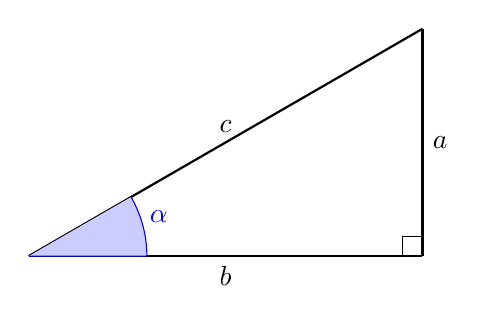
\begin{tikzpicture}[scale=5]
   \draw[thick,color=black] (0,0) -- node[below] {$b$} (1,0);
   \draw[thick,color=black] (1,0) -- node[right] {$a$} (1,0.57735);
   \draw[thick,color=black] (1,0.57735) -- node[above] {$c$} (0,0);
   \filldraw[fill=blue!20!white,draw=blue] (0,0) -- (0.3,0) arc (0:30:0.3); 
   \node[color=blue] at (0.33,0.1) {$\alpha$};
   \draw (0.95,0) -- (0.95,0.05) -- (1,0.05);
   \end{tikzpicture}
   
   \medskip
   
   \begin{tabular}{lll}
   $\sin(\alpha) = \nicefrac{a}{c}$ & $\cos(\alpha) = \nicefrac{b}{c}$ & $\tan(\alpha) = \nicefrac{a}{b}$\\[1ex]
   $\csc(\alpha) = \nicefrac{c}{a}$ & $\sec(\alpha) = \nicefrac{c}{b}$ & $\cot(\alpha) = \nicefrac{b}{a}$  \\
   \end{tabular}

\section*{Trigonometric Identities}
\vspace{-0.05in}
\begin{minipage}[c]{2.0in}

\vspace{-0.335in}
\begin{align*}
&\sin(x)^2 + \cos(x)^2 =1 \\
&2 \cos(x)^2 =  1 + \cos(2 x)\\
&2 \sin(x)^2 = 1 - \cos(2 x)\\
 &\sin\left(x +  y\right) =\sin (x) \cos (y) + \cos (x) \sin (y) \\
&\cos\left(x+y\right)=\cos (x) \cos (y) - \sin (x) \sin (y)    
\end{align*}
\end{minipage}




\section*{Famous Triangles}

\subsection*{The 30-60-90 triangle}

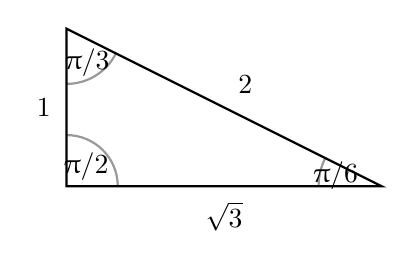
\begin{tikzpicture}[thick]
\coordinate (O) at (0,0);
\coordinate (A) at (4,0);
\coordinate (B) at (0,2);
\draw (O)--(A)--(B)--cycle;

\tkzLabelSegment[below=2pt](O,A){$\sqrt{3}$}
\tkzLabelSegment[left=2pt](O,B){$1$}
\tkzLabelSegment[above right=2pt](A,B){2}

\tkzMarkAngle[fill= orange,size=0.65cm,%
opacity=.4](A,O,B)
\tkzLabelAngle[pos = 0.35](A,O,B){$\uppi/2$}

\tkzMarkAngle[fill= orange,size=0.8cm,%
opacity=.4](B,A,O)
\tkzLabelAngle[pos = 0.6](B,A,O){$\uppi/6$}

\tkzMarkAngle[fill= orange,size=0.7cm,%
opacity=.4](O,B,A)
\tkzLabelAngle[pos = 0.5](O,B,A){$\uppi/3$}



\end{tikzpicture}

\subsection*{The 45-45-90 triangle}


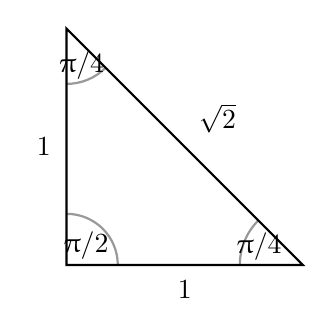
\begin{tikzpicture}[thick]
\coordinate (O) at (0,0);
\coordinate (A) at (3,0);
\coordinate (B) at (0,3);
\draw (O)--(A)--(B)--cycle;

\tkzLabelSegment[below=2pt](O,A){$1$}
\tkzLabelSegment[left=2pt](O,B){$1$}
\tkzLabelSegment[above right=2pt](A,B){$\sqrt{2}$}
\tkzMarkAngle[fill= orange,size=0.65cm,%
opacity=.4](A,O,B)
\tkzLabelAngle[pos = 0.35](A,O,B){$\uppi/2$}

\tkzMarkAngle[fill= orange,size=0.8cm,%
opacity=.4](B,A,O)
\tkzLabelAngle[pos = 0.6](B,A,O){$\uppi/4$}

\tkzMarkAngle[fill= orange,size=0.7cm,%
opacity=.4](O,B,A)
\tkzLabelAngle[pos = 0.5](O,B,A){$\uppi/4$}


\end{tikzpicture}

\section*{Laws of Cosine \& Sine}
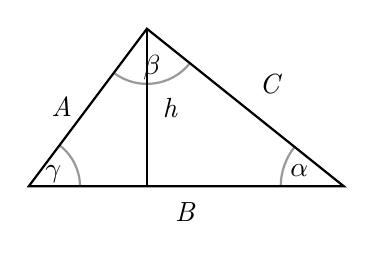
\begin{tikzpicture}[thick]
\coordinate (O) at (0,0);
\coordinate (A) at (4,0);
\coordinate (B) at (1.5,2);
\coordinate (C) at (1.5,0);
\draw (O)--(A)--(B)--cycle;
\draw (C)--(B)--cycle;

\tkzLabelSegment[below=2pt](O,A){\textit{B}}
\tkzLabelSegment[left=2pt](O,B){\textit{A}}
\tkzLabelSegment[above right=2pt](A,B){\textit{C}}
\tkzLabelSegment[right=2pt](C,B){\textit{h}}
\tkzMarkAngle[fill= orange,size=0.65cm,%
opacity=.4](A,O,B)
\tkzLabelAngle[pos = 0.35](A,O,B){$\gamma$}

\tkzMarkAngle[fill= orange,size=0.8cm,%
opacity=.4](B,A,O)
\tkzLabelAngle[pos = 0.6](B,A,O){$\alpha$}

\tkzMarkAngle[fill= orange,size=0.7cm,%
opacity=.4](O,B,A)
\tkzLabelAngle[pos = 0.5](O,B,A){$\beta$}


\end{tikzpicture}

\subsection*{Law of cosines}
\[
    C^2 = A^2 + B^2 - 2 A B \cos(\gamma) 
\]

\subsection*{Law of sines}
\[
    \frac{\sin{\alpha}}{A} =  \frac{\sin{\beta}}{B} =  \frac{\sin{\gamma}}{C}
\]

\subsection*{Area}

\[
    \mbox{Area} = h B / 2=  A B \sin(\gamma) /2
\]


\section*{Solution of equations}
\vspace{-0.2in}
\subsubsection*{Algebraic}
\vspace{-0.2in}
\begin{minipage}[c]{0.1666666666667\textwidth}
\begin{align*}
& \big [a b = 0 \big ] \equiv \big [ a = 0 \mbox{ \textbf{or} } b = 0 \big ]\\
& \big [ a^2 = b^2 \big ] \equiv \big [ a = b \mbox{ \textbf{or} } a = -b \big ]\\
&\left [ \frac{a}{b} = 0 \right ] \equiv \big [ a = 0 \mbox{ \textbf{and} } b \neq 0 \big ] \\
&\left [\frac{a}{b} = \frac{c}{d}  \right ] \equiv \big [ad  = bc \mbox{ \textbf{and}  } b \neq 0  \mbox{ \textbf{and}  }  d \neq 0 \big ] \\
&\big [|a| = |b|  \big ] \equiv \big [a =b \mbox{ \textbf{or} } a = -b \big ]\\
&\big [ \sqrt{a}  = b \big ] \equiv \big [a = b^2 \mbox{ \textbf{and}  } b \ge 0 \big ] \\
\intertext{For \(a \neq 0\),}
& \big [a x^2 + b x + c = 0 \big] \equiv \left [x = \frac{-b \pm \sqrt{b^2 - 4 a c}}{2 a} \right] \\
\end{align*}
\end{minipage}
\vspace{-0.4in}
\subsubsection*{Trig}
\vspace{-0.2in}
\begin{minipage}[c]{0.1666666666667\textwidth}
\begin{align*}
&\big [\cos(a) = 0 \big ]  \equiv  \big [a =  (k - 1/2)  \uppi, k \in \integers \big ]\\
&\big [\sin(a) = 0 \big ]  \equiv  \big [ a = k \uppi, k \in \integers \big ] \\
&\big [\tan(a) = 0 \big ]  \equiv  \big [ a = k \uppi, k \in \integers \big ] \\
%&\big [\sin(a) = b  \big] \equiv \big [a = \sin^{-1}(b) + 2 k \uppi  \mbox{ \textbf{or} } [a = \sin^{-1}(b) + 2 k \uppi \big ]
\end{align*}
\end{minipage}

\end{multicols*}


\newpage

\begin{comment}
\subsubsection*{Trig (continued)}

$\big [\sin(a) = b  \big] \equiv \begin{cases} a = \sin^{-1}(b) + 2 k \uppi  \mbox{ \textbf{or} } a = -\sin^{-1}(b) + (2 k + 1) \uppi \big ] &\mbox{ if } b \in [-1,1] \\
  \varnothing  & \mbox{ if } b \notin [-1,1] \end{cases}$
\end{comment}

\section*{Graphs}
\vspace{-0.2in}
\subsubsection*{Cosine, sine, and tangent}
\vspace{-0.2in}
\begin{figure}[h]
\centering
\begin{minipage}{.333\textwidth}
  \centering
  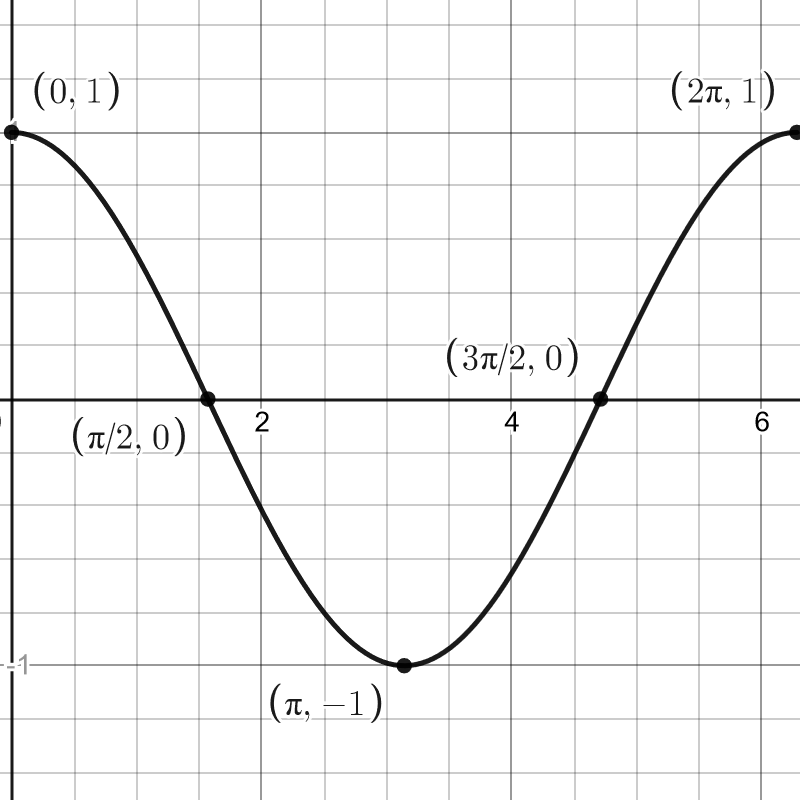
\includegraphics[width=.25\linewidth]{desmos-graph-cos}
  \captionof{figure}{Graph of $y = \cos(x)$ on $[0, 2\uppi]$.}
  %\label{fig:test1}
\end{minipage}%
\begin{minipage}{.333\textwidth}
  \centering
  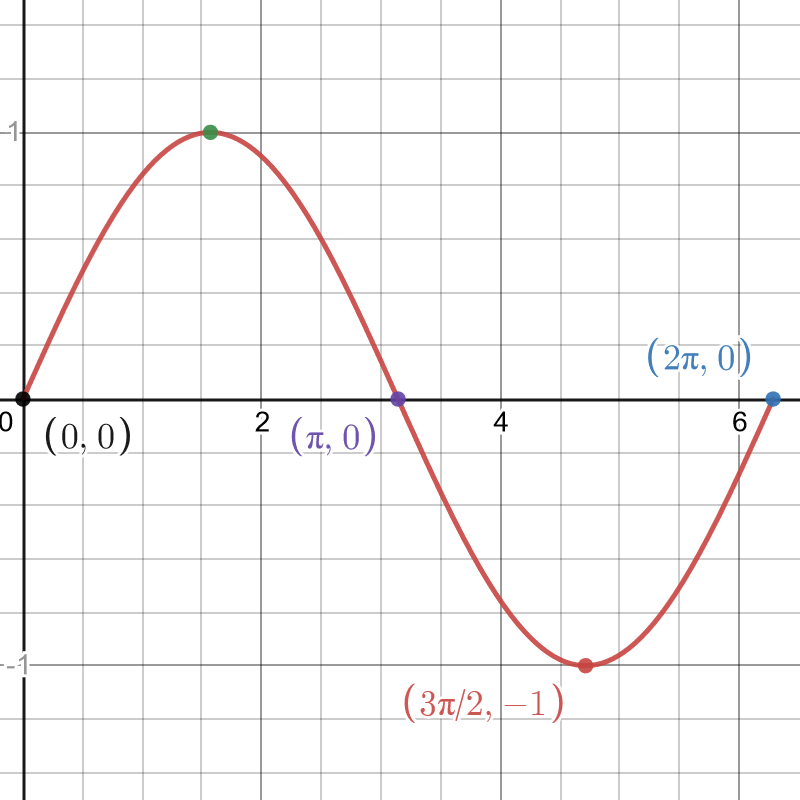
\includegraphics[width=.25\linewidth]{desmos-graph-sine}
  \captionof{figure}{Graph of $y = \sin(x)$ on $[0, 2\uppi]$.}
  %\label{fig:test2}
\end{minipage}%
\begin{minipage}{.333\textwidth}
  \centering
  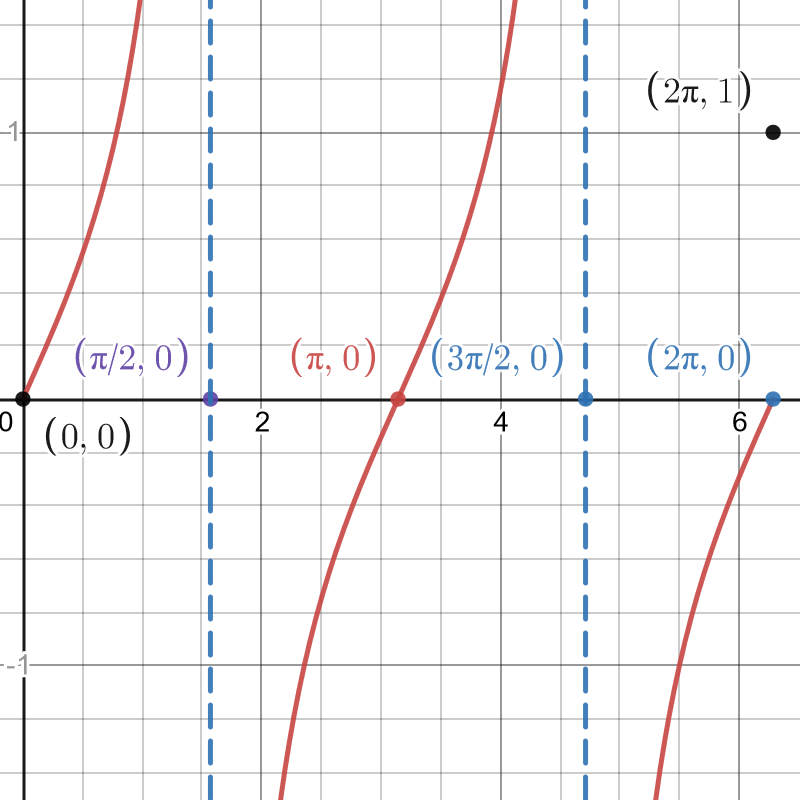
\includegraphics[width=.25\linewidth]{desmos-graph-tan}
  \captionof{figure}{Graph of $y = \tan(x)$ on $[0, 2\uppi]$.}
  %\label{fig:test2}
\end{minipage}
\end{figure}
\vspace{-0.2in}
\subsubsection*{Arccosine, arcsine, and arctangent}
\vspace{-0.2in}
\begin{figure}[h]
\centering
\begin{minipage}{.333\textwidth}
  \centering
  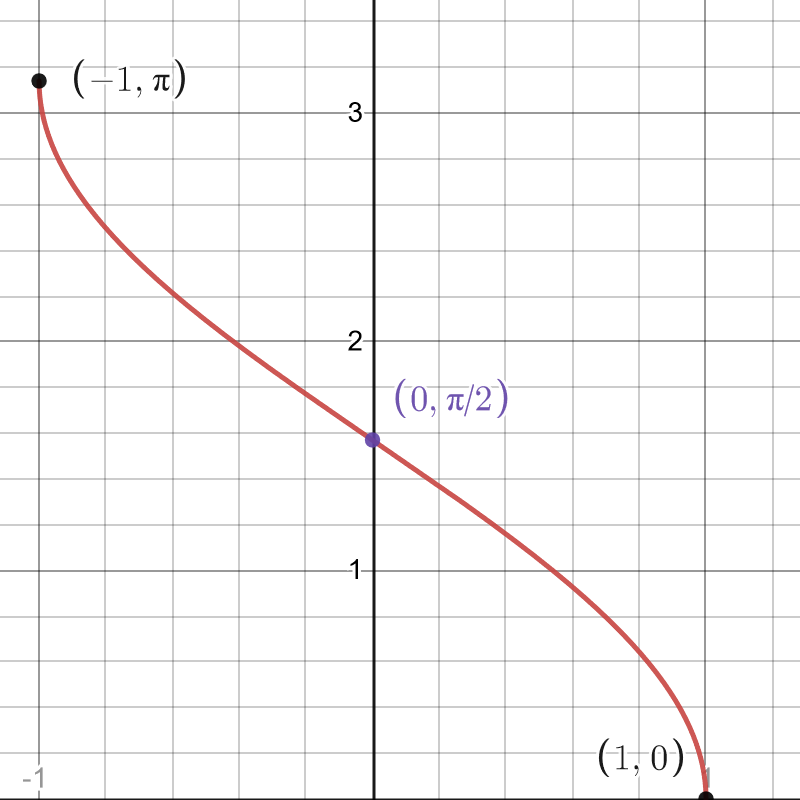
\includegraphics[width=.25\linewidth]{desmos-graph-invcos}
  \captionof{figure}{Graph of $y = \arccos(x)$ on $[-1,1]$.}
  %\label{fig:test1}
\end{minipage}%
\begin{minipage}{.333\textwidth}
  \centering
  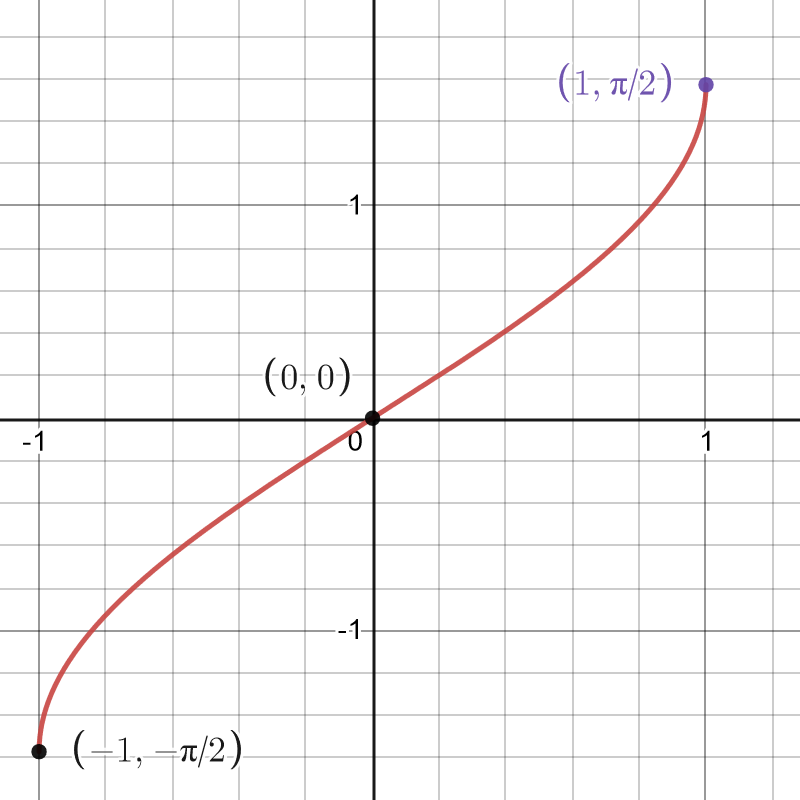
\includegraphics[width=.25\linewidth]{desmos-graph-invsin}
  \captionof{figure}{Graph of $y = \arcsin(x)$ on $[-1,1]$.}
  %\label{fig:test2}
\end{minipage}%
\begin{minipage}{.333\textwidth}
  \centering
  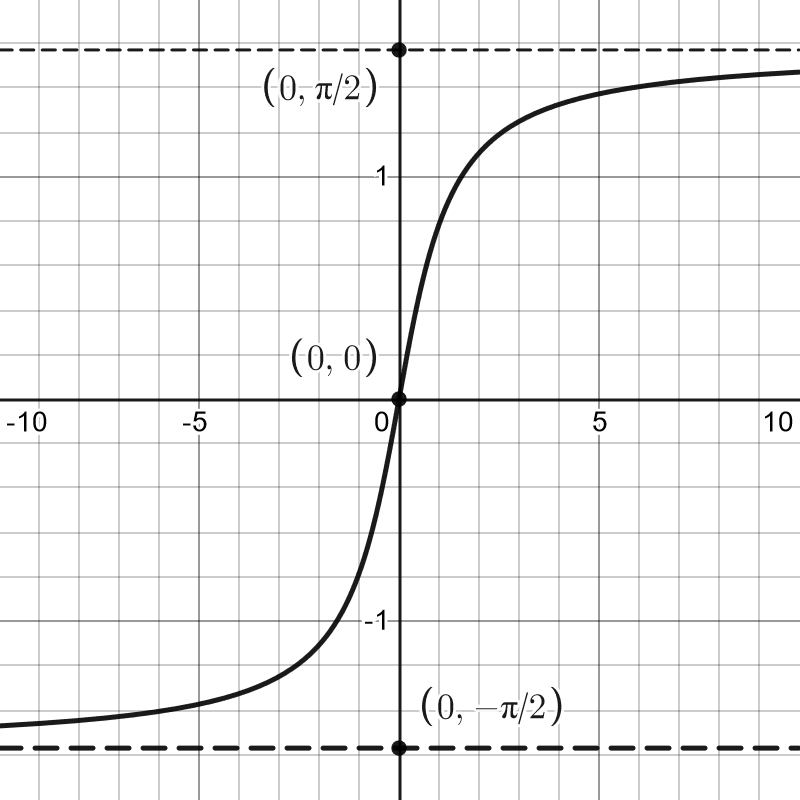
\includegraphics[width=.25\linewidth]{desmos-graph-invtan}
  \captionof{figure}{Graph of $y = \arctan(x)$ on $[-10,10]$.}
  %\label{fig:test2}
\end{minipage}
\end{figure}
\begin{comment}

\begin{figure}[h]
\centering
\begin{minipage}{.333\textwidth}
  \centering
  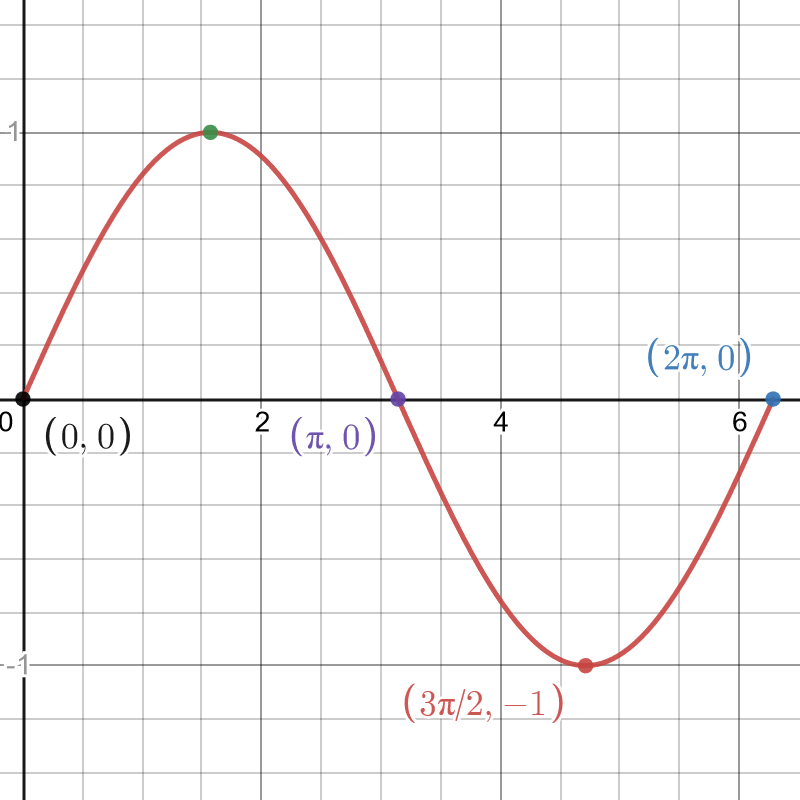
\includegraphics[width=.333\linewidth]{desmos-graph-sine}
  \captionof{figure}{Graph of $y = \sin(x)$ on $[0, 2\uppi]$.}
  %\label{fig:test1}
\end{minipage}%
\begin{minipage}{.333\textwidth}
  \centering
  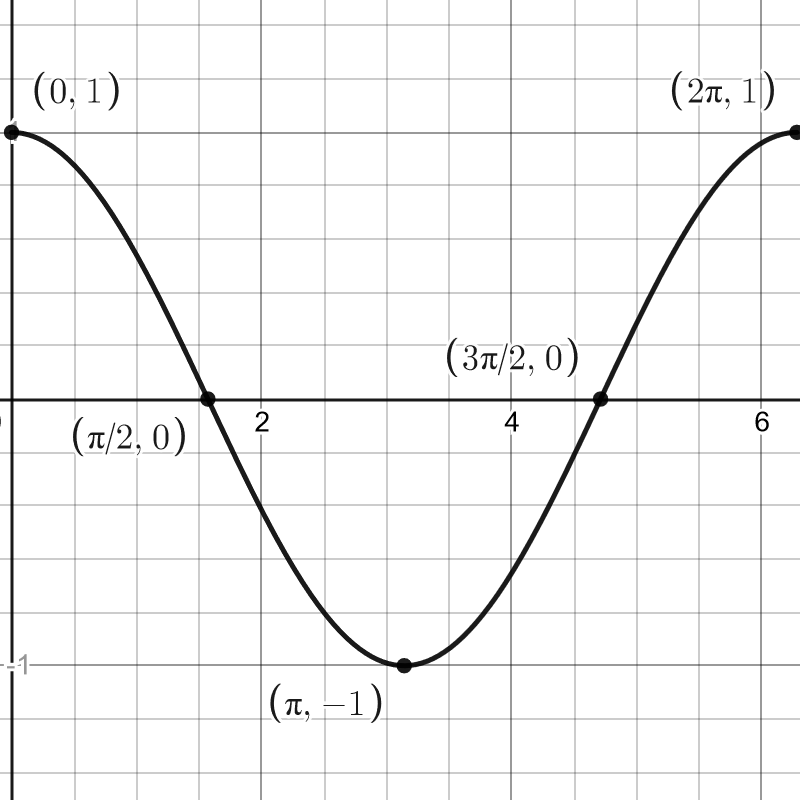
\includegraphics[width=.3\linewidth]{desmos-graph-cos}
  \captionof{figure}{Graph of $y = \cos(x)$ on $[0, 2\uppi]$.}
  %\label{fig:test2}
\end{minipage}%
\begin{minipage}{.333\textwidth}
  \centering
  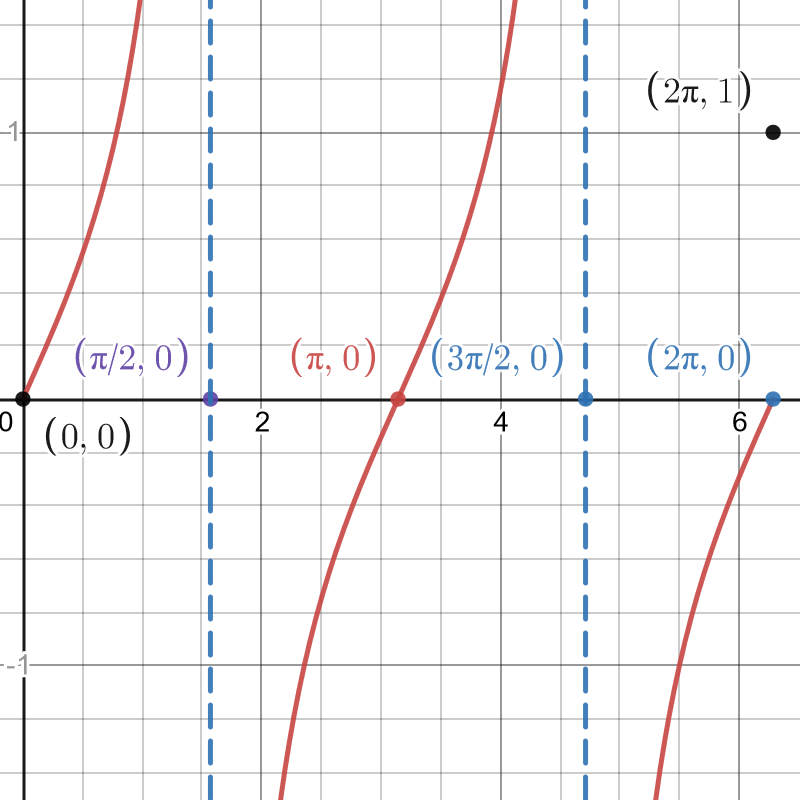
\includegraphics[width=.3\linewidth]{desmos-graph-tan}
  \captionof{figure}{Graph of $y = \tan(x)$ on $[0, 2\uppi]$.}
  %\label{fig:test2}
\end{minipage}
\end{figure}
\begin{figure}[h]
\centering
\begin{minipage}{.333\textwidth}
  \centering
  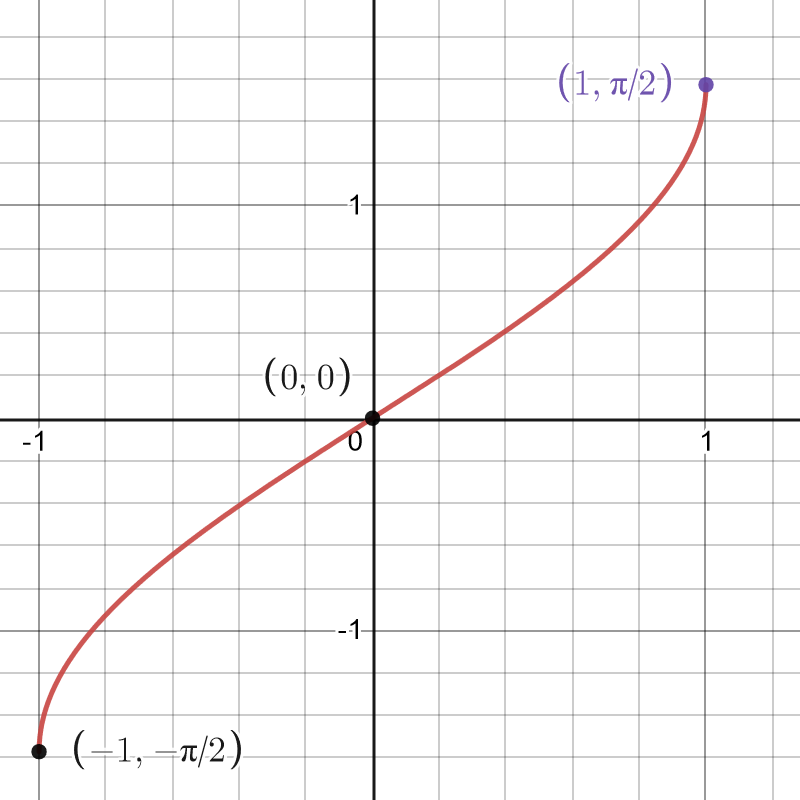
\includegraphics[width=.333\linewidth]{desmos-graph-invsin}
  \captionof{figure}{Graph of $y = \sin(x)$ on $[0, 2\uppi]$.}
  %\label{fig:test1}
\end{minipage}%
\begin{minipage}{.333\textwidth}
  \centering
  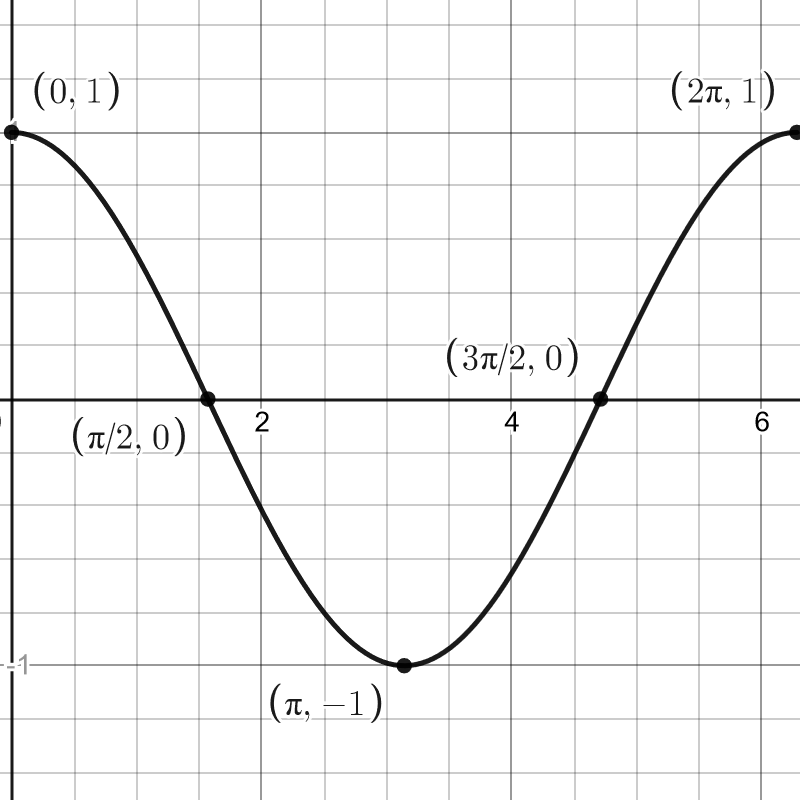
\includegraphics[width=.3\linewidth]{desmos-graph-cos}
  \captionof{figure}{Graph of $y = \cos(x)$ on $[0, 2\uppi]$.}
  %\label{fig:test2}
\end{minipage}%
\begin{minipage}{.333\textwidth}
  \centering
  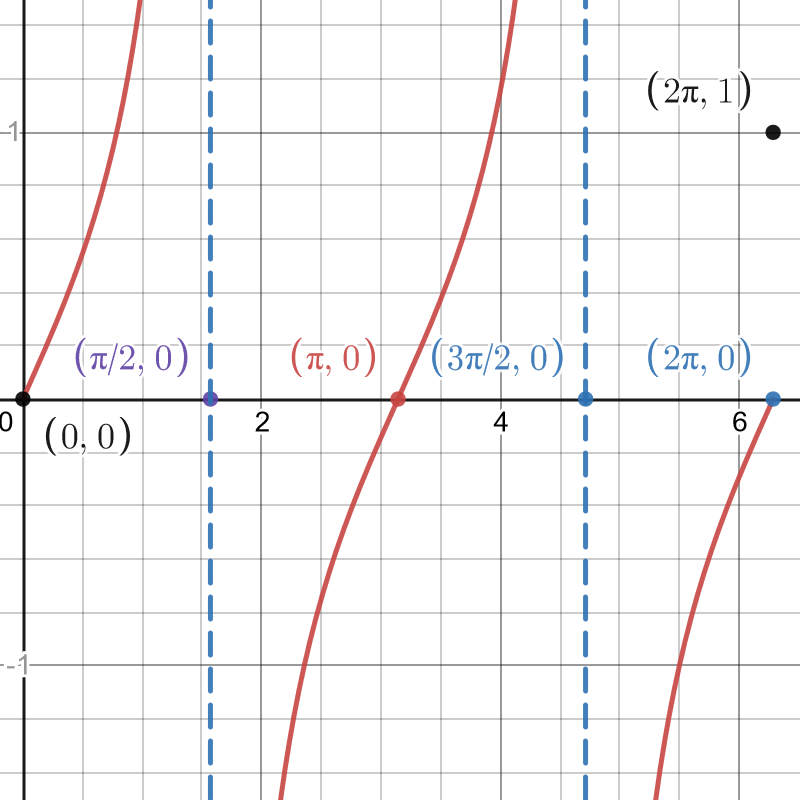
\includegraphics[width=.3\linewidth]{desmos-graph-tan}
  \captionof{figure}{Graph of $y = \tan(x)$ on $[0, 2\uppi]$.}
  %\label{fig:test2}
\end{minipage}
\end{figure}
\end{comment}

\begin{comment}
\fbox{
 \begin{tikzpicture}[>=stealth]
  \begin{axis}[
      xmin=-4,xmax=4,
      ymin=-1.5,ymax=1.5,
      axis x line=middle,
      axis y line=middle,
      axis line style=<->,
      xlabel={$x$},
      ylabel={$y$},
      ]
      \addplot[no marks,blue,<->] expression[domain=-pi:pi,samples=100]{cos(deg(x))} 
                  node[pos=0.65,anchor=south west]{$y=\cos(x)$}; 
  \end{axis}
\end{tikzpicture}}

\fbox{
\begin{tikzpicture}[>=stealth]
  \begin{axis}[
      xmin=-4,xmax=4,
      ymin=-1.5,ymax=1.5,
      axis x line=middle,
      axis y line=middle,
      axis line style=<->,
      xlabel={$x$},
      ylabel={$y$},
      ]
      \addplot[no marks,blue,<->] expression[domain=-pi:pi,samples=100]{sin(deg(x))} 
                  node[pos=0.65,anchor=south west]{$y=\sin(x)$}; 
  \end{axis}
\end{tikzpicture}}
\fbox{
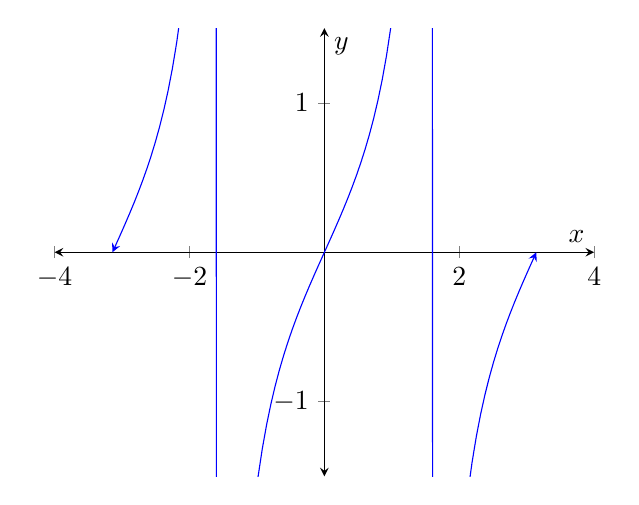
\begin{tikzpicture}[>=stealth]
  \begin{axis}[
      xmin=-4,xmax=4,
      ymin=-1.5,ymax=1.5,
      axis x line=middle,
      axis y line=middle,
      axis line style=<->,
      xlabel={$x$},
      ylabel={$y$},
      ]
      \addplot[no marks,blue,<->] expression[domain=-pi:pi,samples=100]{tan(deg(x))} 
                  node[pos=0.15,anchor=south west]{$y=\tan(x)$}; 
  \end{axis}
\end{tikzpicture}}

\end{comment}

\section*{Unit Circle}

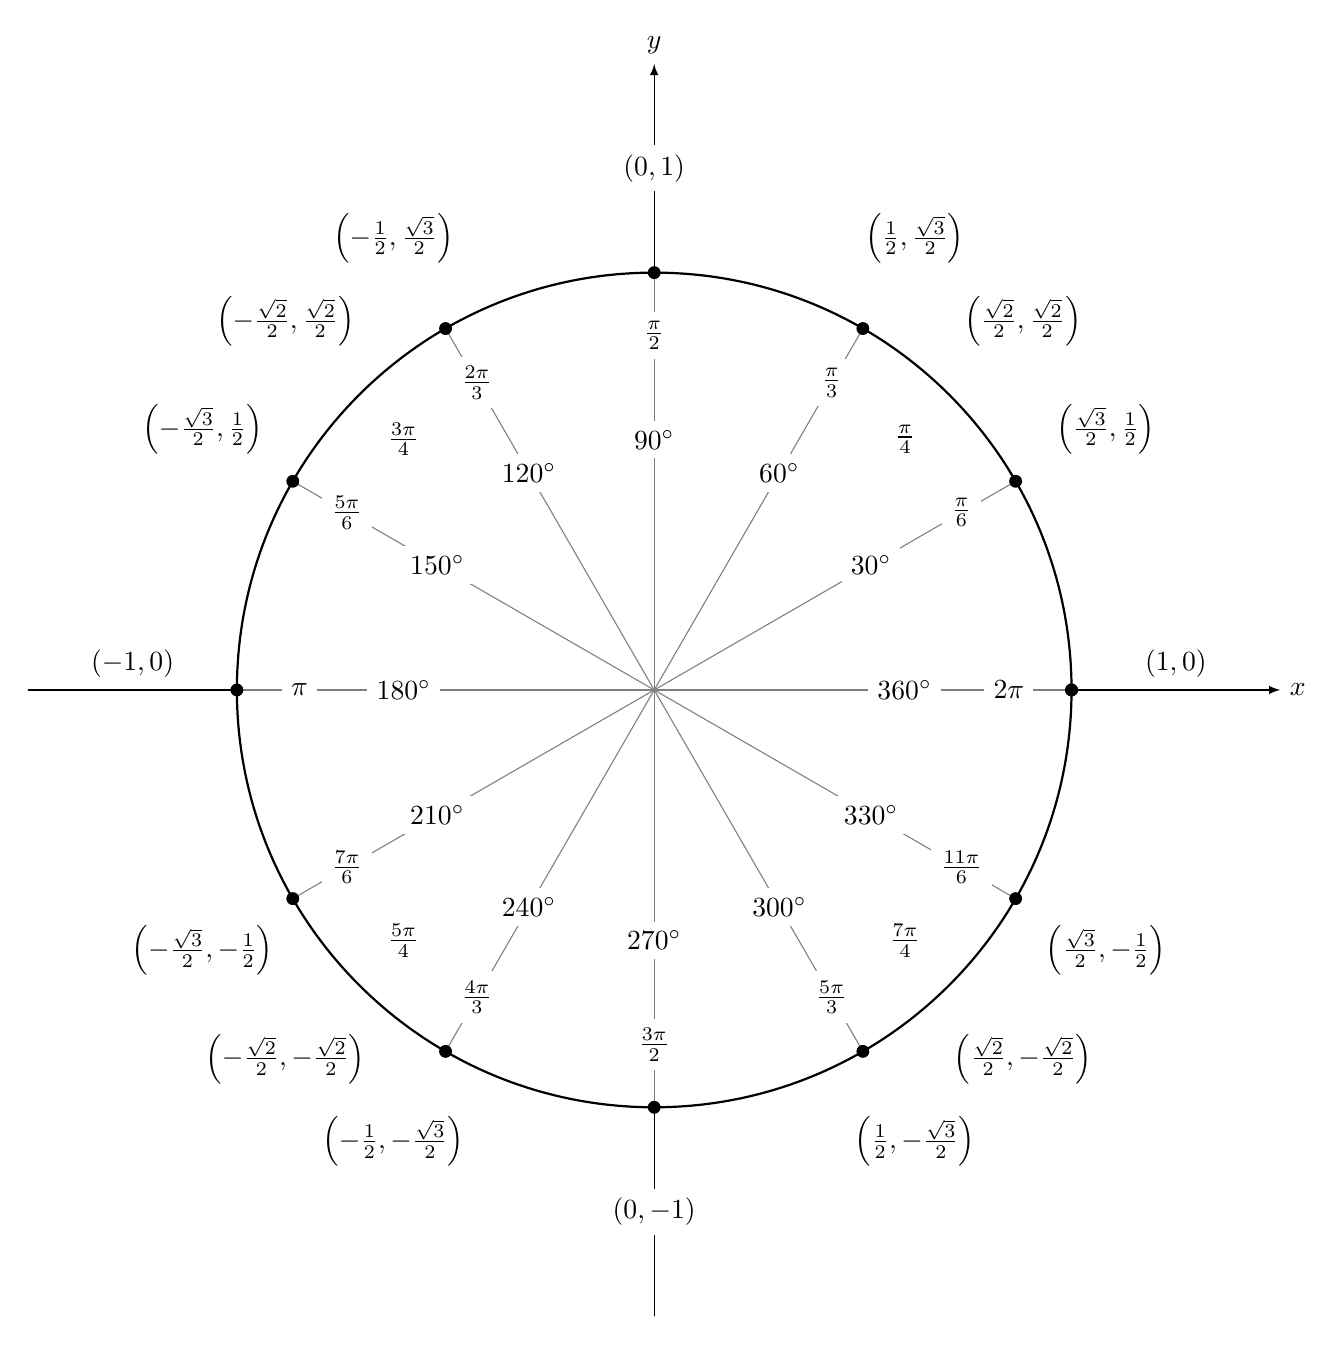
\begin{tikzpicture}[scale=5.3,cap=round,>=latex]
    % draw the coordinates
    \draw[->] (-1.5cm,0cm) -- (1.5cm,0cm) node[right,fill=white] {$x$};
    \draw[->] (0cm,-1.5cm) -- (0cm,1.5cm) node[above,fill=white] {$y$};

    % draw the unit circle
    \draw[thick] (0cm,0cm) circle(1cm);

    \foreach \x in {0,30,...,360} {
            % lines from center to point
            \draw[gray] (0cm,0cm) -- (\x:1cm);
            % dots at each point
            \filldraw[black] (\x:1cm) circle(0.4pt);
            % draw each angle in degrees
            \draw (\x:0.6cm) node[fill=white] {$\x^\circ$};
    }

    % draw each angle in radians
    \foreach \x/\xtext in {
        30/\frac{\pi}{6},
        45/\frac{\pi}{4},
        60/\frac{\pi}{3},
        90/\frac{\pi}{2},
        120/\frac{2\pi}{3},
        135/\frac{3\pi}{4},
        150/\frac{5\pi}{6},
        180/\pi,
        210/\frac{7\pi}{6},
        225/\frac{5\pi}{4},
        240/\frac{4\pi}{3},
        270/\frac{3\pi}{2},
        300/\frac{5\pi}{3},
        315/\frac{7\pi}{4},
        330/\frac{11\pi}{6},
        360/2\pi}
            \draw (\x:0.85cm) node[fill=white] {$\xtext$};

    \foreach \x/\xtext/\y in {
        % the coordinates for the first quadrant
        30/\frac{\sqrt{3}}{2}/\frac{1}{2},
        45/\frac{\sqrt{2}}{2}/\frac{\sqrt{2}}{2},
        60/\frac{1}{2}/\frac{\sqrt{3}}{2},
        % the coordinates for the second quadrant
        150/-\frac{\sqrt{3}}{2}/\frac{1}{2},
        135/-\frac{\sqrt{2}}{2}/\frac{\sqrt{2}}{2},
        120/-\frac{1}{2}/\frac{\sqrt{3}}{2},
        % the coordinates for the third quadrant
        210/-\frac{\sqrt{3}}{2}/-\frac{1}{2},
        225/-\frac{\sqrt{2}}{2}/-\frac{\sqrt{2}}{2},
        240/-\frac{1}{2}/-\frac{\sqrt{3}}{2},
        % the coordinates for the fourth quadrant
        330/\frac{\sqrt{3}}{2}/-\frac{1}{2},
        315/\frac{\sqrt{2}}{2}/-\frac{\sqrt{2}}{2},
        300/\frac{1}{2}/-\frac{\sqrt{3}}{2}}
            \draw (\x:1.25cm) node[fill=white] {$\left(\xtext,\y\right)$};

    % draw the horizontal and vertical coordinates
    % the placement is better this way
    \draw (-1.25cm,0cm) node[above=1pt] {$(-1,0)$}
          (1.25cm,0cm)  node[above=1pt] {$(1,0)$}
          (0cm,-1.25cm) node[fill=white] {$(0,-1)$}
          (0cm,1.25cm)  node[fill=white] {$(0,1)$};
\end{tikzpicture}







\vfill
%\tiny
\noindent For an extensive list of trigonometric function facts, see \url{https://dlmf.nist.gov/4.14}.

\noindent Revised 8 August 2021. Barton Willis is the author of this work. It 
licensed under CC0 1.0 (\url{https://creativecommons.org/publicdomain/zero/1.0 }).

  
\end{document}
